\documentclass[11pt]{report}

\usepackage[utf8]{inputenc}
\usepackage{geometry}
\geometry{hmargin=1cm,vmargin=2cm}
\usepackage{xspace}
\usepackage[toc,page]{appendix} 
\usepackage[pdftex]{graphicx}
\usepackage{tikz}
\usepackage{tikz-uml}
\usepackage{lscape}
\setlength{\columnseprule}{0.5pt}
 \parskip=10pt
\usepackage{sidecap}
\usepackage{wrapfig}
\usepackage{pgfkeys}
\usepackage{array}
\usepackage{tkz-graph}
\usetikzlibrary{arrows}
\usetikzlibrary{positioning}
\usepackage[francais]{babel}
\usepackage[T1]{fontenc}
\usepackage[bookmarks={true},bookmarksopen={true}]{hyperref}
\usepackage{multicol}
\usepackage{fancyhdr}
\usepackage[babel=true]{csquotes}
\usepackage{url} % Pour écrire des adresses cliquables.
\usepackage{lmodern} % Pour changer le pack de police.
\usepackage{etoolbox}
\usepackage{colortbl}
\usepackage[final]{pdfpages} 
\usepackage{titlesec}
\usepackage{multirow}
\newcommand{\chapterP}{\chapter}
\pagestyle{fancy}
\usepackage{caption}
\usepackage{indentfirst}
\setlength{\parindent}{15pt}


\captionsetup[table]{labelformat=empty}
\renewcommand{\headrulewidth}{1pt}
\fancyhead[L]{La Pastourelle}
\fancyhead[C]{}
\fancyhead[R]{\leftmark}
\renewcommand{\footrulewidth}{1pt}
\fancyfoot[L]{IUT de Rodez}
\fancyfoot[C]{- \thepage -}
\fancyfoot[R]{2015 - 2016}

\usepackage[light,math]{iwona}

\setcounter{secnumdepth}{5}
\renewcommand{\thechapter}{\Alph{chapter}}
\renewcommand{\thesection}{\Alph{chapter}.\Roman{section})}
\renewcommand{\thesubsection}{\Alph{chapter}.\Roman{section}.\arabic{subsection})}
\renewcommand{\thesubsubsection}{\Alph{chapter}.\Roman{section}.\arabic{subsection}.\alph{subsubsection})}
\parskip 5pt

\tikzstyle{line}=[-, thick]


\title{Projet Externe\\La Pastourelle}
\author{DEMERY Cyril\\COSTA Mickael\\MEJANE Thibault\\ZEGHMATI Clément}
\date{2015-2016}

\pdfinfo{%
  /Title    (Projet Web - La Pastourelle)
  /Author   (DEMERY Cyril)
  /Creator  (DEMERY Cyril)
  /Producer ()
  /Subject  (La Pastourelle)
  /Keywords ()
}

\begin{document}
\maketitle
\setcounter{tocdepth}{5}
%SS\tableofcontents
\chapter{Plan de Management de Projet}
\section{Introduction}
L'assocation La Pastourelle est une assocation de danses folkloriques 
aveyronnaises. Ce site est destiné aux membres de l'assocation mais aussi aux 
visiteurs externes qui souhaitent suivre les actualités concernant les 
évènements à venir. Il sera donc régulièrement mis à jour par les ayants 
droits de l'assocation. Par conséquent, il faudra que le site soit à la fois 
agréable pour les visiteurs, mais aussi pour toutes les personnes qui 
s'occupent de la mise en forme du contenu.\\

\par Ce dossier est le Plan de Management de Projet, c'est lui qui regroupera 
tous les choix stratégiques sur la manière dont le projet sera conduit : 
l'organisation de l'équipe, la gestion des tâches ainsi que le cahier des 
charges, après une analyse approfondie des besoins du client.

\section{Présentation}
\subsection{Les acteurs}
Ce projet consistera à dialoguer avec une association, et plus particulièment 
avec les personnes suivantes : 
\begin{itemize}
    \item Mr Pagès, secrétaire adjoint de l'assocation\\
\end{itemize}

\par A l'IUT, nos interlocuteurs sont Mr. Belières qui s'occupe de superviser 
l'avancement du projet et de nous aider dans nos éventuels choix techniques, 
ainsi que Mr. Rous qui est chargé du suivi de la gestion de projet.   \\

\par Concernant notre équipe, elle est formé de quatre étudiants de deuxième 
année informatique : 
\begin{itemize}
    \item Mickael Costa
    \item Cyril Démery
    \item Thibault Méjane
    \item Clément Zeghmati
\end{itemize}


\subsection{Enjeux et bénéfices}
Ce projet possède de multiple enjeux. Tout d'abord, le fait de travailler pour 
une association nous impose de fournir un résultat afin de représenter au mieux 
le travail de l'IUT et le sérieux de ces étudiants. Ensuite, travailler pour 
un acteur extérieur, non-scolaire et non-informaticien, est un challenge car il 
faudra utiliser des supports de communication adaptés afin de se faire 
comprendre. \\

\par Concernant l'aspect technique, ce projet ne peut être que bénéfique car il 
va nous apprendre à travailler sur un existant déjà bien établit. Ainsi, il va 
falloir se plonger dans un code qui nous est étranger. Aussi, développer une 
application Web, en l'occurence un site internet, est un plus car c'est une 
domaine en pleine expansion actuellement.\\

\par Enfin, nous pouvons dire que cette expérience sera facilement visible par 
des personnes extérieurs et pourra ainsi nous aider dans la recherche d'un 
emploi.
\subsection{Cahier des charges}
L'équipe projet s'engage à réaliser les taches suivantes :
\subsubsection*{Tâches prioritaires}
Elles sont obligatoires et sont la cause de la rénovation du site, elles doivent être menées à terme en priorité. 

Correction des erreurs graves liées à l'administration :
\begin{itemize}
\item Membre qui ne bascule pas dans l'annuaire après sa validation par un
administrateur
\item Problème de masque de saisie qui empêche de voir l'intégralité du contenu
à modifier 
\item Problème de saisie de la phrase du jour qui ne fonctionne pas en saisie
directe, mais seulement via un copié/collé depuis Word
\item Erreur de caractère dans le planning : impossible de supprimer ou de
modifier un événement contenant un caractère invalide
\end{itemize}

\subsubsection*{Tâches importantes}
Ces tâches seront réalisées dans un second temps et s'il est possible de les effectuer 
sans trop toucher à la structure du site.
\begin{itemize}
 \item Version multilingue du site : il faut, en plus de l'espagnol, donner la
possibilité d'ajouter du texte en anglais et en occitan 
 \item Ajout de vidéos : donner la possibilité d'intégrer des liens youtube
 \item Dimensionnement automatique des photos : réduire automatiquement la
taille des images, soit à une taille saisie, soit à une taille par défaut 
 \item Changer l'ordre d'affichage des revues
 \item Revoir la carte du monde : corriger le problème de doublon et de
placement du drapeau, ou intégrer un nouveau système de localisation d’évènements
 \item Changement du formulaire de la page des actualités : il faudrait unifier
 les champs afin de ne pas avoir à saisir trop d'informations inutiles
 \item Enlever la mention \og pièce jouée \fg automatique pour la partie théâtre
 qui s'intègre automatiquement si l'on saisit quelque chose
\end{itemize}


\subsubsection*{Tâches secondaires}
Ces éléments sont facultatifs et seront réalisés en fonction de nos disponibilités et du temps restant.
\begin{itemize}
\item Changer la couleur de fond : mettre des couleurs plus modernes
\item Changer les icônes : là aussi, intégrer des éléments plus agréables à
regarder
\item Inclure un responsive design afin de faciliter la navigation depuis
différents supports
\item Repenser le bon de commande afin de le rendre plus attractif
\item Ergonomie et présentation (liens, boutons de connexion, etc, style de
formulaire) afin de faciliter la navigation et l'accès au contenu
\item Changer les photos de la boutique avec des photos plus récentes
\item Inclure un captcha pour éviter des attaques de robots qui ont déjà eu lieu
dans le passé
\end{itemize}

\subsection{Charte du projet}
Le but de ce projet est de pouvoir fournir un site fonctionnel à la MOA, 
correspondant aux exigences initiales en ce qui concerne la mise à jour des 
informations ou bien encore le multilangage, tout en fournissant une 
ergonomie facilitant la visite de personnes externes.\\

\par Pour apprécier ce projet, le client pourra s'appuyer sur les éléments 
suivants : 
\begin{itemize}
    \item Les livrables fournis sont en adéquation avec le cahier des charges
    \item Les engagements initiaux en ce qui concerne la documentation ont été 
tenus
    \item Les livrables exigés ont tous été fournis\\
\end{itemize}

\par L'objectif de ce projet est d'introduire un mode de formation, voire 
d'auto-formation, proche de celui que l'on retrouve en entreprise. C'est pour 
cela qu'il est nécessaire de travailler de façon méthodique et rigoureuse. 
Ainsi, le chef de projet sera chargé de veiller au bon respect des points 
précédents, ainsi qu'à celui des échéances, devra coordonner les différents 
acteurs et sera l'interlocuteur entre le groupe et les acteurs externes.\\

\par En plus du chef de projet, nous nous sommes appuyés sur deux autres rôles 
pour coordonner l'équipe : 
\begin{itemize}
    \item Le gestionnaire de configuration qui s'occupe de gérer les différents 
version du site, des versions des logiciels de chacun, de la sauvegarde des 
informations en cas de soucis, et des choix d'outils de travail.
    \item Le secrétaire dont le but est de garder tous les documents relatifs 
au projet à jour, ainsi que de rédiger les comptes rendus de réunion\\
\end{itemize}

\par Concernant les différents livrables à fournir, nous devons rendre : 
	\begin{itemize}
	  \item le site hébergé, testé et fonctionnel
	  \item un manuel d'utilisateur pour l'assocation
	  \item un dossier projet, avec les schémas de conception et les codes d'accès pour modifier le site web
	  \item un plan projet
	\end{itemize}


\section{Organisation}
\subsection{Grandes étapes}
Ce projet est particulier car il ne dure qu'un semestre, et par conséquent en 
l'ayant commencé mi-octobre et devant le rendre mi-décembre, il ne durera que 
deux mois. \\
\par Nous allons toutefois essayer de le scinder en deux, avec une première 
partie de réponse aux exigences de l'assocation, et une seconde partie basée 
sur des améliorations non-proposées mais envisageable.

Nous avons dû réaliser divers documents afin d'assurer le suivi de projet : 
\begin{itemize}
    \item La liste des tâches
    \item Le Gantt
    \item La répartition des tâches
    \item Les comptes rendus de réunion \\
\end{itemize}

\subsection{Rôles}
En ce qui concerne la gestion des rôles pour ce projet, nous avons choisit de 
les fixer dès le début et au vu de la durée du projet, de ne pas les modifier, 
ainsi on obtient le tableau suivant :  
\par
\begin{tabular}{ | c | c | }
\hline 
   COSTA Mickael & Pas de rôle  \\ \hline 
   DEMERY Cyril & Chef de Projet / Gestionnaire de configuration \\ \hline 
   MEJANE Thibault & Secrétaire de projet \\ \hline 
   ZEGHMATI Clément & Pas de rôle \\ \hline
 \end{tabular}
\subsection{Méthodes de suivi de projet}
Nous avons décidé de suivre un modèle en V, car le projet est trop court pour 
des itérations de 3 semaines, et ainsi nous pouvons tester les fonctionnalités 
au fûr et à mesure qu'elles sont implantées.
\begin{figure}[htp] \centering{
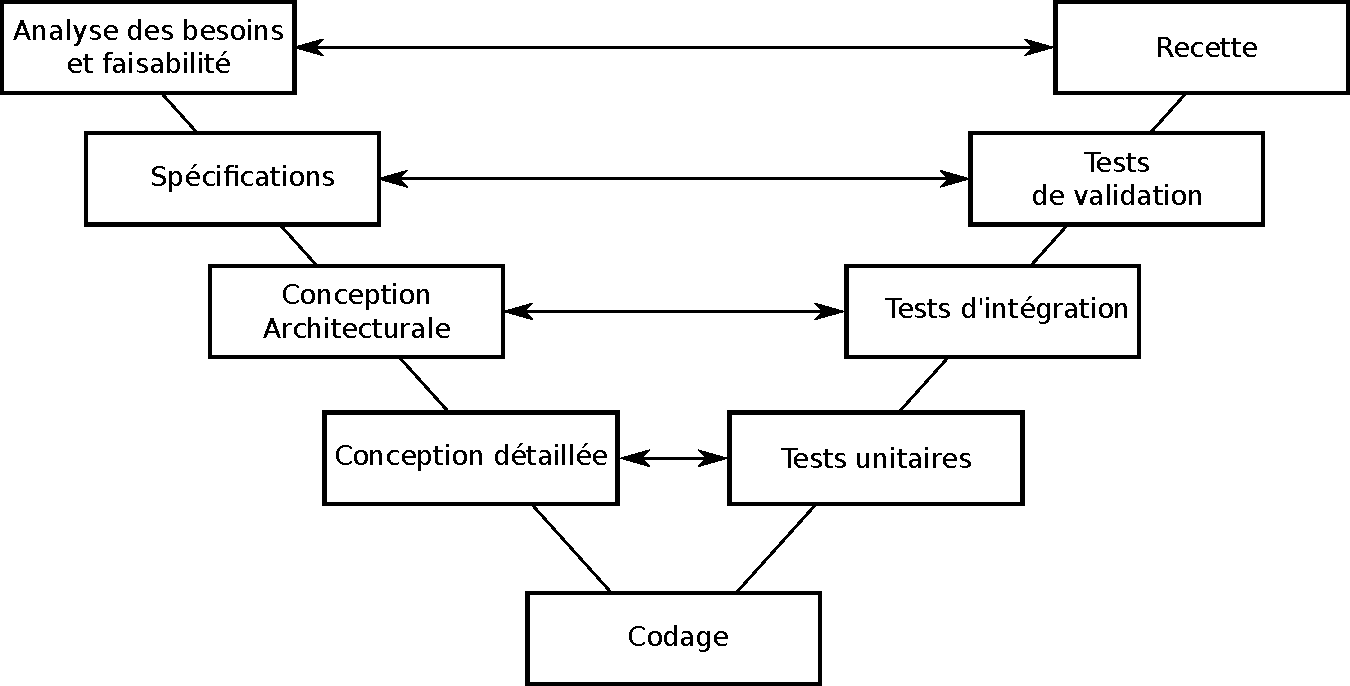
\includegraphics[scale=0.60]{include/cycle_v.pdf}}
\caption{Modèle en V}
\end{figure}

\subsection{Plan de communication}
Durant les périodes scolaires, nous sommes tous présents sur Rodez, mais étant 
donné que pendant les vacances et les week-end nous rentrons dans nos 
départements respectifs, il devient tout de suite plus difficile de communiquer.
C'est pourquoi nous avons décidé d'utiliser Skype combiné à TeamViewer. Ces 
deux outils nous permettent de travailler en binôme quelque soit la distance, 
et ainsi de pouvoir intéragir avec le reste du groupe.\\
\par Toutefois, nous devons nous réunir régulièrement afin de définir la 
stratégie à suivre et de programmer les réunions avec les différents 
intervenants. A ce titre, il serait pertinent de rencontrer la MOA mi-octobre, 
puis début novembre et enfin vers le 20-25 novembre afin de l'informer 
de l'anvancée du projet et d'établir les divers travaux à effectuer.
\newpage

\subsection{Modèles de documents}
\begin{figure}[htp] \centering{
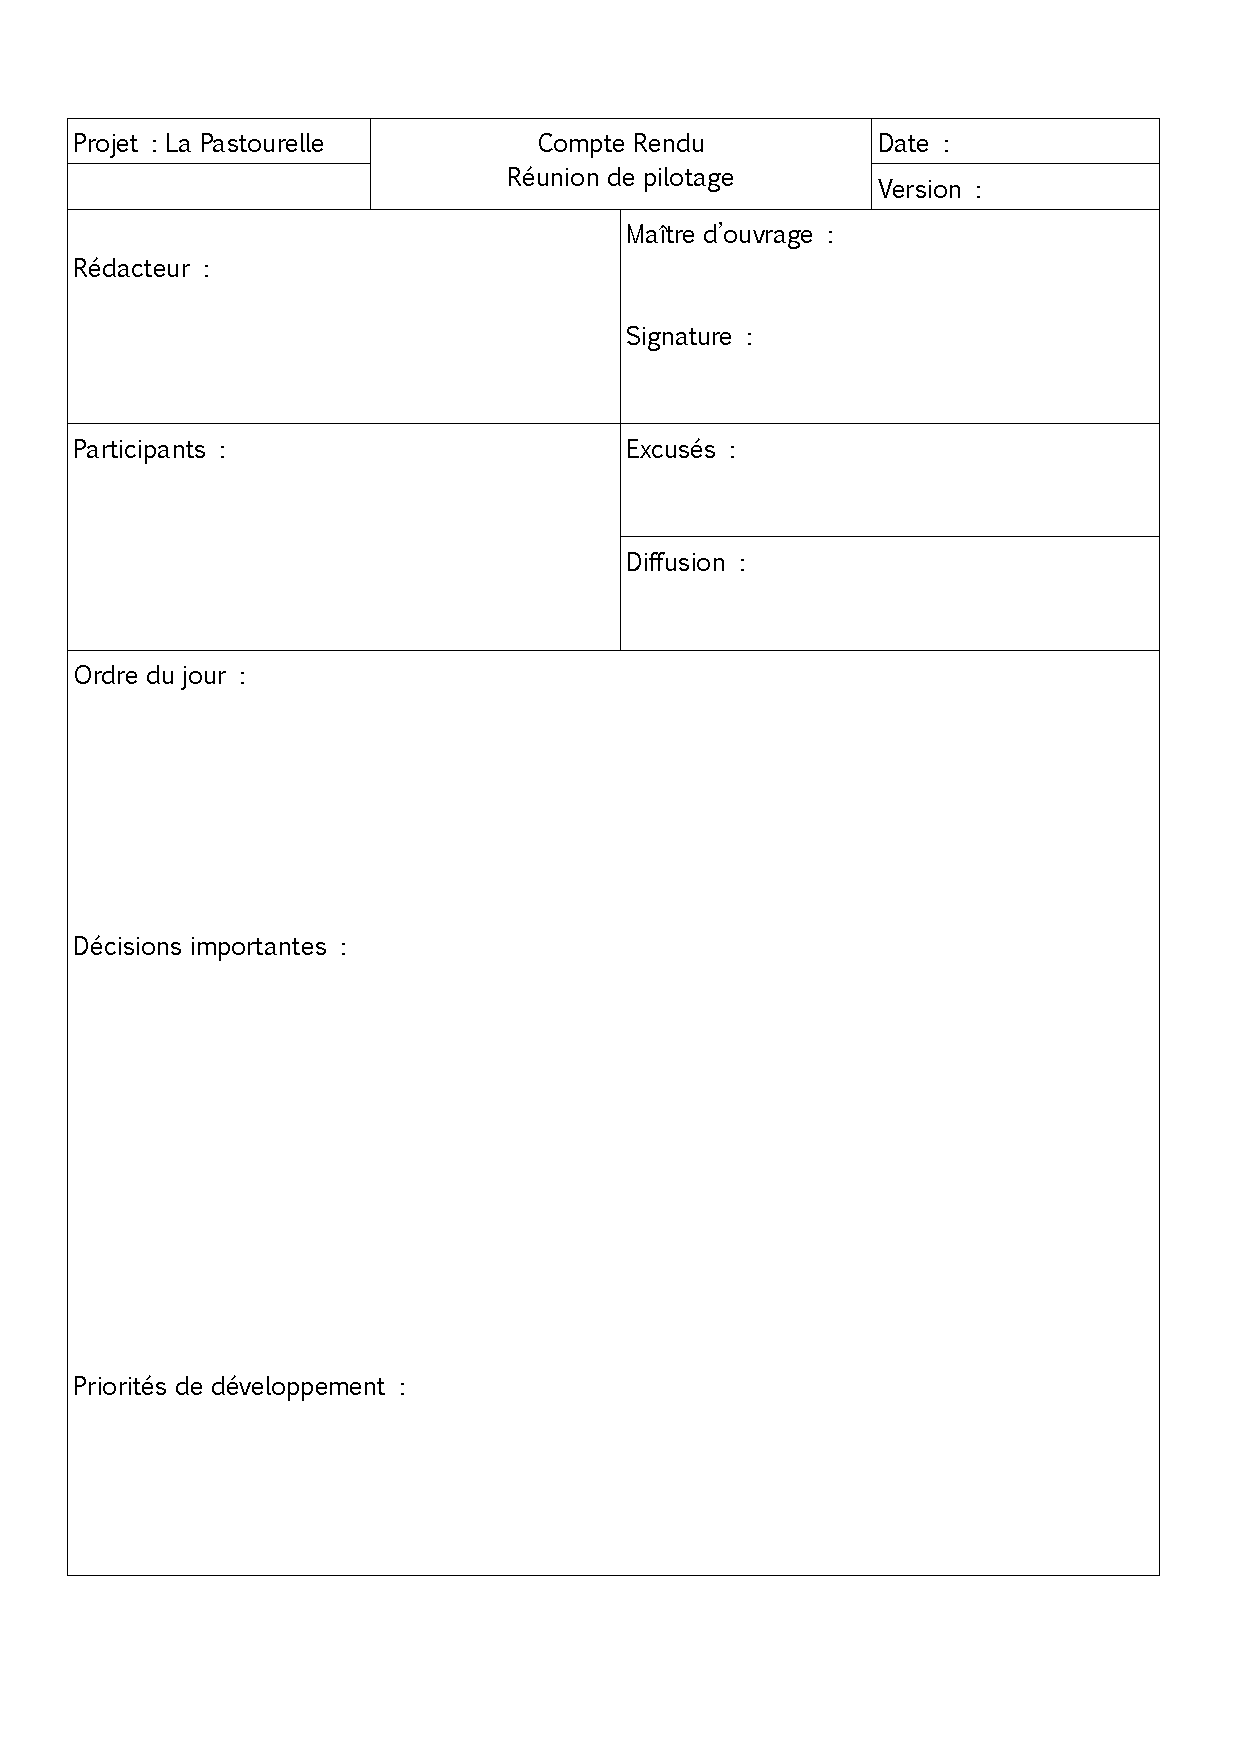
\includepdf[scale=0.80]{include/copil_template.pdf}}
\caption{Modèle de COPIL}
\end{figure}
\newpage
\begin{figure}[htp] \centering{
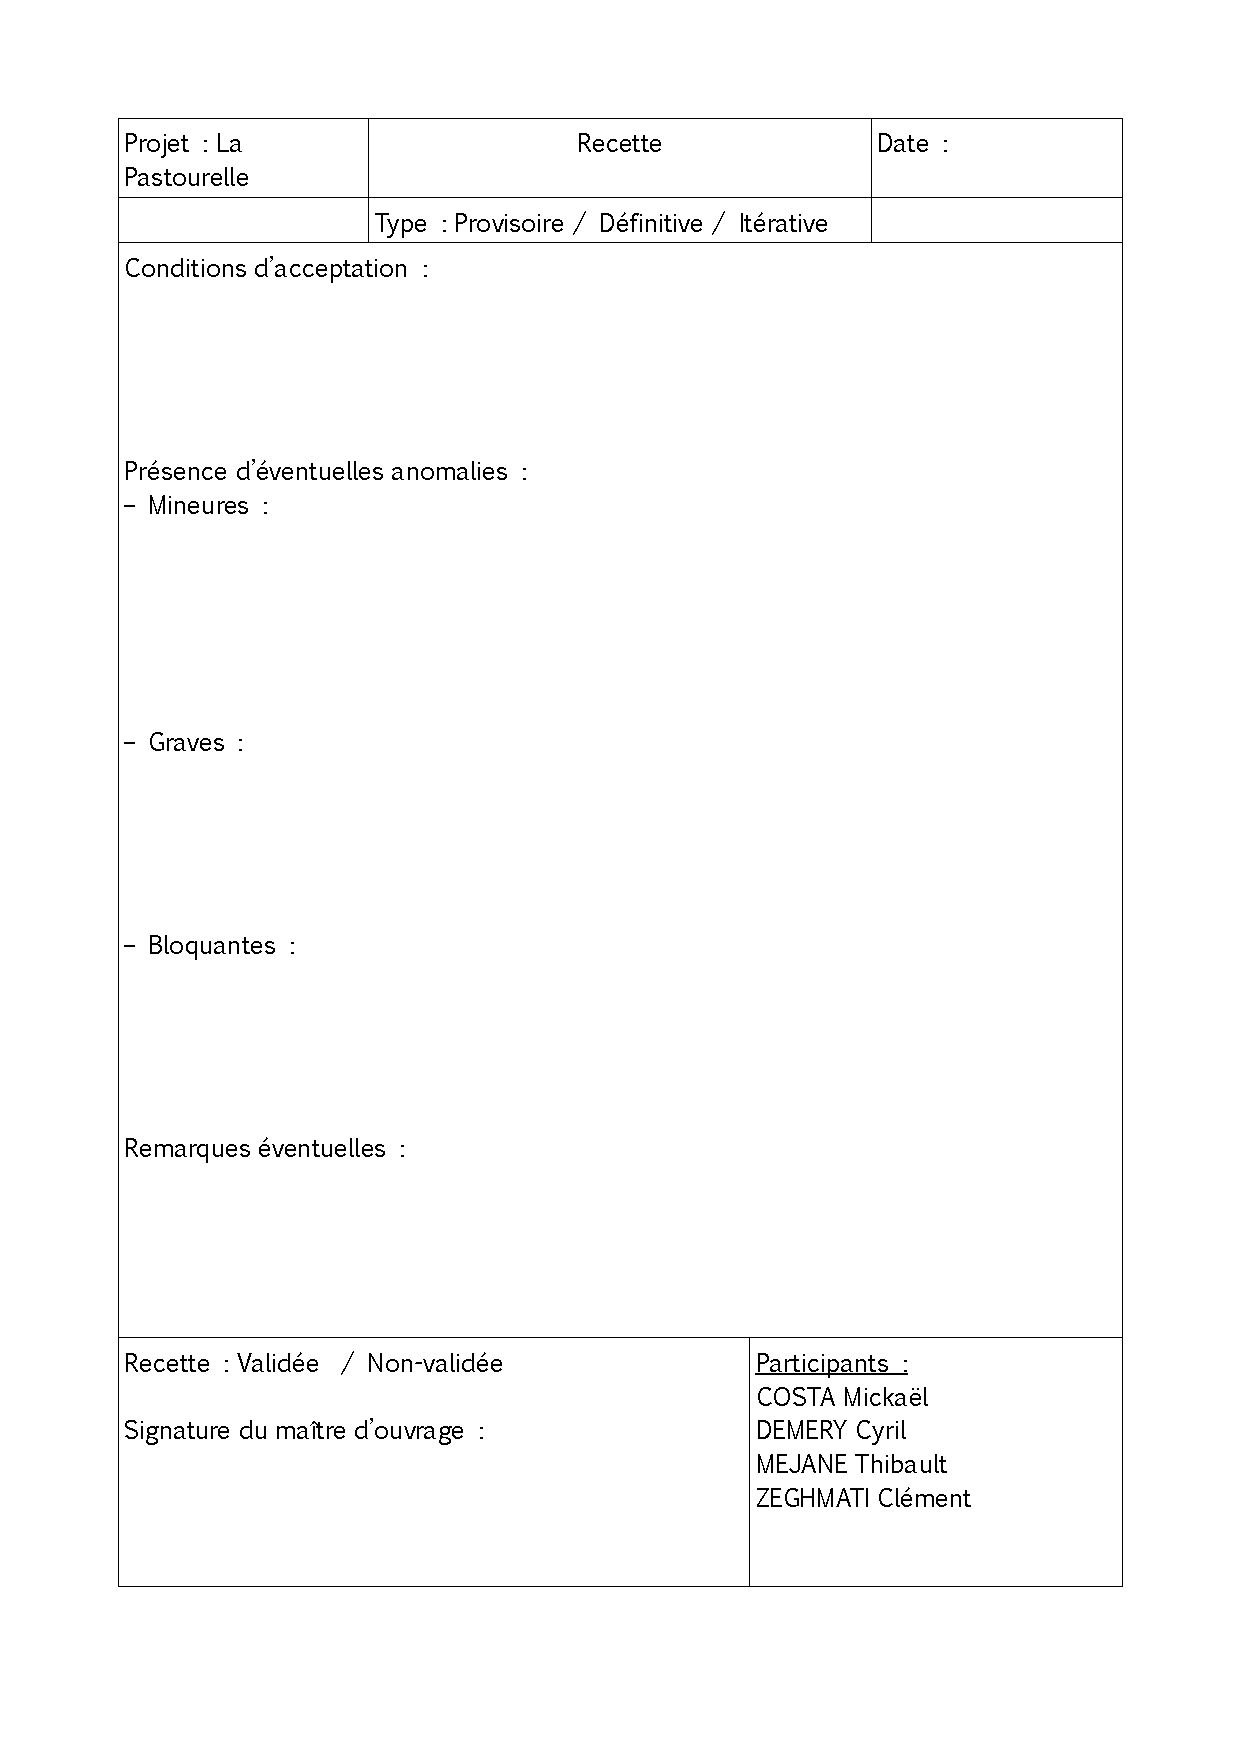
\includepdf[scale=0.80]{include/recette_template.pdf}}
\caption{Modèle de recette}
\end{figure}
\newpage

\subsection{Comité de pilotage}

\subsection{Gestion de la configuration}
Pour ce projet, le gestionnaire de configuration, Cyril, a décidé d'utiliser
les logiciels suivants : \\ 
\par 
\begin{tabular}{ | c | c | c | }
\hline 
   Logiciel & Version & Plugin  \\ \hline 
   LaTeX & 2.22 & tickzuml \\ \hline 
   LibreOffice & 4.2.8 & spellchecker \\ \hline 
   Eclipse PHP & Luna & texclipse, egit, pdf4linux \\ \hline
   PHP & 5.6 & PDO \\ \hline
   Apache & 2 & \\ \hline
   MySQL & 5.6.27 & \\ \hline
   PhpMyAdmin & 4.5 & \\ \hline
 \end{tabular}
 
 \par En ce qui concerne le travail collaboratif, les codes sources seront
 hébergés sur GitHub de manière à pouvoir les manipuler facilement depuis
 n'importe où, et de toujours conserver la dernière version stable. Pour la
 partie gestion de la plannification, nous utilisons Redmine installé en SaaS
 sur OpenShift afin de pouvoir consulter les tâches à effctuer depuis n'importe
 où, ainsi qu'accéder à la dernière version des documents projets, même si le
 rapport est hébergé sur Github.
 \par Github est un système d'hébergement de code source public dans la version 
 que nous allons utiliser, par conséquent, les codes sources seront visibles 
 par tout internaute. Il ne pourra toutefois les modifier. Ainsi par raison de
 sécurité, nous avons retiré les outils permettant à un tiers d'accéder aux
 données privées de l'association ainsi qu'aux informations concernant les
 membres.
 \par Les rapports seront rédigés la plupart du temps en LaTeX afin de
 s'affranchir du système d'exploitation, car certains utilisent Linux et
 d'autres Windows. 

\section{Pilotage}
 Une réunion projet est le moment où l'on pose des questions à la MOA afin de
s'assurer du travail à accomplir, ou de proposer des éléments de réalisation.
 Un comité de pilotage (COPIL) a pour but de faire le point à un instant T sur
l'avancée du projet et définir les taches qui devront etre accomplis dans le futur. \\

 \par Nous nous engageons à rencontrer le client plusieurs fois durant le
 projet. Tout d'abord avant les vacances de Toussaint afin d'éclaircir les
 taches à accomplir durant une réunion projet. Ensuite, nous le rencontrerons
 autour de mi-novembre pour un COPIL qui portera sur les exigences du client qui
 ont été accomplis jusqu'à présent (taches urgentes et importantes). 
 \par Enfin, il
 faudra faire un dernier comité de pilotage le 8 ou le 9 décembre afin de
 présenter les scénarios de test, les modifications effectuées, établir la
recette et les conditions de migration.
\section{Recettes}
 La recette est l'acception du projet par le client. Pour cela, il est
nécessaire d'établir des conditions préalables à la signature de celle-ci : \\
\begin{itemize}
 \item les erreurs bloquantes : ce sont celles qui empechent l'accès au site.
 En cas d'erreur bloquante, la recette ne pourra pas etre signée. \\
  \item les erreurs importantes : celles qui empechent un module de fonctionner,
  mais qui ne perturbe pas l'intégralité ni la stabilité du site. Nous nous
 autorisons un maximum de deux erreurs de ce type pour signer la recette. \\
  \item les erreurs minimes : celles qui sont relatives à l'aspect général du
  site, elles n'empechent en rien le fonctionnement. Le recette ne sera pas
  signée si plus de dix erreurs minimes sont détectées. \\
\end{itemize}

\par Pour signer la recette, tous les livrables exigés devront impérativement
etre fournis.

\section{Migration}
 En ce qui concerne la migration du site et de sa base de données associée, nous
 nous engageons à déployer la version à jour sur le serveur existant, en
 assurant la sauvegarde des versions précédentes. Nous testerons également
 l'ensemble des fonctionnalités sur le nouveau site afin de s'assurer que tout
 est déployé correctement.
 Une fois le site déployé, nous signerons une nouvelle recette afin d'assurer
que tout a été correctement implémenté.

\newpage
\section{Plannification}
\subsection{Prévision initiale}
Initialement, nous avions prévus de suivre cette plannification, avec la
première partie jusqu'au jalon définie avec un peu de précision, puis la suite
beaucoup moins car nous devions faire le point avec le client pour voir si le
résultat de la première partie lui convenait.
\par

\begin{tabular}{ | c | p{4cm} | c | c | c | c | c | c |   }
\hline 
Id & Tâche & Statut & Priorité & Estimée (h) & Début & Fin & Réalisé \\ \hline

%prio urgente %
4 & Caractères indésirables dans le planning & A réaliser & Urgente & 5 & 21/10/15
	& 03/11/15 & 0  \\ \hline
3 & Saisie de la phrase du jour & A réaliser & Urgente & 2 & 21/10/15 & 03/11/15
	& 0  \\ \hline
2 & Correction du masque de saisie & A réaliser & Urgente & 3 & 21/10/15 &
	03/11/15 & 0  \\ \hline
	
%prio haute %	
14 & Correction de l'ajout des pièces de théâtre & A réaliser & Haute & 2 &
	13/11/15 & 09/12/15 & 0 \\ \hline
13 & Changement du formulaire de la page d'actualité & A réaliser & Haute & 3 &
	21/10/15 & 11/11/15 & 0  \\ \hline
12 & Revoir la carte du monde & A réaliser & Haute & 3 & 21/10/15 & 11/11/15 & 0
	 \\ \hline
11 & Changer l'ordre d'affichage des revues & A réaliser & Haute & 1 & 21/10/15
	& 11/11/15 & 0  \\ \hline
10 & Dimensionnement automatique des photos & A réaliser & Haute & 1 & 21/10/15
	& 03/11/15 & 0  \\ \hline
9 & Ajout de vidéos & A réaliser & Haute & 1 & 21/10/15 & 03/11/15 & 0  \\
\hline
7 & Version multilingue & A réaliser & Haute & 20 & 21/10/15 & 03/11/15 & 0  \\
\hline
6 & Erreur de validation & A réaliser & Haute & 3 & 21/10/15 & 03/11/15 & 0  \\
\hline


%prio moyenne%

	
%prio basse%	
20 & Inclure un captcha & A réaliser & Basse & ? & 13/11/15 &
	09/12/15 & 0  \\ \hline
19 & Revoir l'ergonomie et la présentation & A réaliser & Basse & ? & 13/11/15
	& 09/12/15 & 0  \\ \hline
18 & Changer les photos de la boutique & A réaliser & Basse & ? & 13/11/15 &
	09/12/15 & 0  \\ \hline
17 & Repenser le bon de commande & A réaliser & Basse & ? & 13/11/15 & 09/12/15
	& 0  \\ \hline
16 & Inclure un responsive design & A réaliser & Basse & ? &
	13/11/15 & 09/12/15 & 0  \\ \hline
15 & Changer la couleur de fond & A réaliser & Basse & ? & 13/11/15 & 09/12/15
	& 0   \\ \hline
8 & Changer les icones & A réaliser & Basse & ? & 21/10/15 & 09/12/15 & 0  \\
\hline

	
	% Total %
 & Total estimé &  &  & 44 &  &  & \\ \hline
 \end{tabular}

 \begin{landscape}
   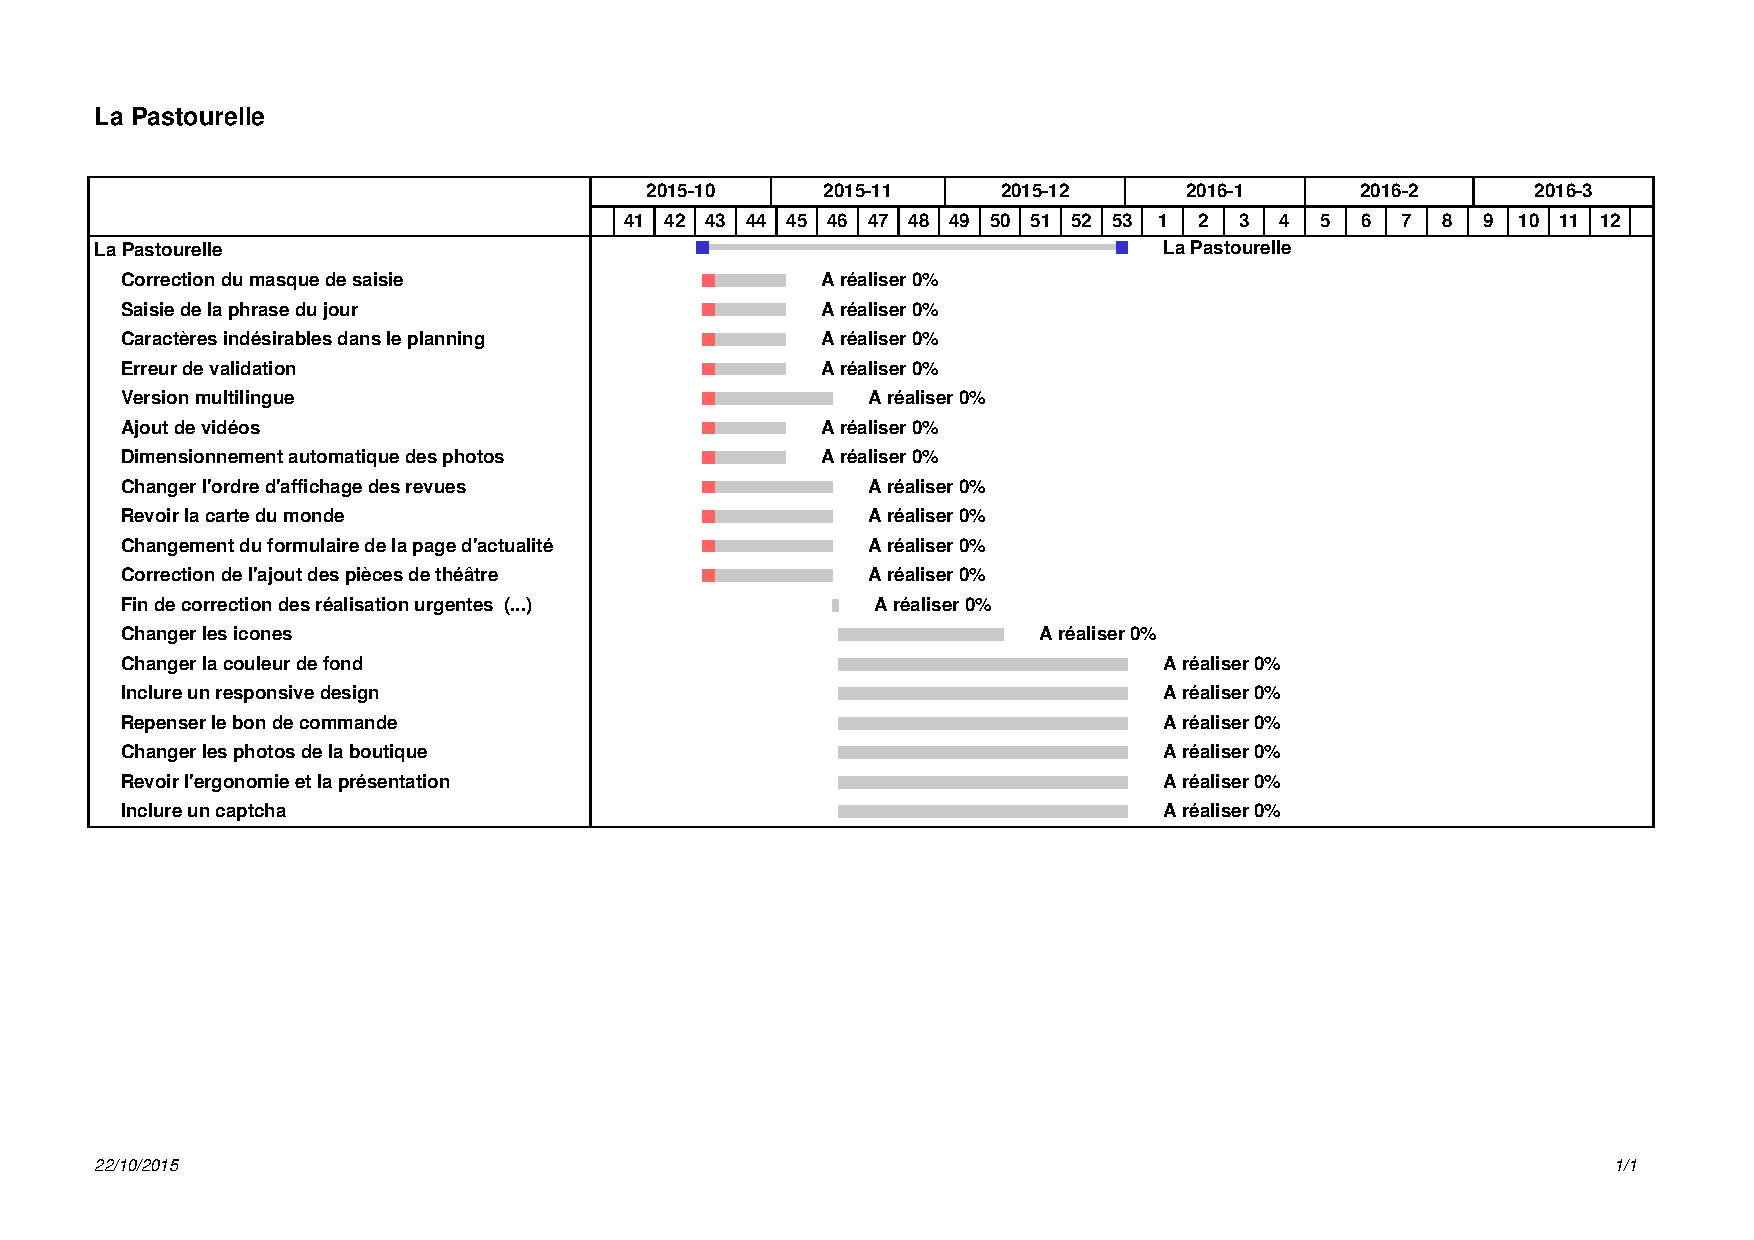
\includepdf{include/gantt22-10.pdf}
\end{landscape}
\clearpage

\subsection{Evolution de la plannification}
Par la suite, la plannification a évolué, ainsi au 3 novembre 2015, soit juste
après les vacances, il se trouve que nous en étions à ce niveau (voire page
suivante). Ici, nous constatons que la plupart des tâches qui étaient à
effectuer pour le retour des vacances n'ont pas été effectuées et, par
conséquent, nous sommes très en retard sur le planning car nous avions prévus
initialement d'effectuer la démonstration avec le client à la mi-novembre.
\par Toutefois, ce retard s'explique par la grande majorité du groupe débute sur
php et n'est pas capable de développer rapidement, ou de s'intégrer sur une
solution déjà développée comme c'est le cas ici. Toutefois, le but de ce projet
est avant tout que tout le monde participe à son développement, donc nous devons
faire avec et les développeurs les plus habiles doivent aider ceux qui sont en
difficultés. 
\par Par conséquent, il est fortement envisageable que nous nous mettions à
travailler en binôme afin de rattraper le temps perdu.
\begin{tabular}{ | c | p{4cm} | c | c | c | c | c | c | c |  }
\hline 
Id & Tâche & Statut & Priorité & Estimée (h) & Début & Fin & Réalisé &
Préd. \\ \hline

%prio urgente %

22 & Correction encodage & A réaliser & Urgente & 5 & 21/10/15 & 11/11/15 & 0
	 & \\ \hline
4 & Caractères indésirables dans le planning & Terminée & Urgente & 5 & 21/10/15
	& 03/11/15 & 100\% & \\ \hline
3 & Saisie de la phrase du jour & A réaliser & Urgente & 2 & 21/10/15 & 03/11/15
	& 0 & \\ \hline
2 & Correction du masque de saisie & A réaliser & Urgente & 3 & 21/10/15 &
	03/11/15 & 0 & \\ \hline
	
%prio haute %	
21 & Correction de l'inscription & Terminé & Haute & 3 & 21/10/15 &
	11/11/15 & 100\% & \\ \hline
14 & Correction de l'ajout des pièces de théâtre & A réaliser & Haute & 2 &
	13/11/15 & 09/12/15 & 0 & 5 \\ \hline
13 & Changement du formulaire de la page d'actualité & A réaliser & Haute & 3 &
	21/10/15 & 11/11/15 & 0 & \\ \hline
12 & Revoir la carte du monde & A réaliser & Haute & 3 & 21/10/15 & 11/11/15 & 0
	& \\ \hline
11 & Changer l'ordre d'affichage des revues & A réaliser & Haute & 1 & 21/10/15
	& 11/11/15 & 0 & \\ \hline
10 & Dimensionnement automatique des photos & A réaliser & Haute & 1 & 21/10/15
	& 03/11/15 & 0 & \\ \hline
9 & Ajout de vidéos & A réaliser & Haute & 1 & 21/10/15 & 03/11/15 & 0 & \\
\hline
7 & Version multilingue & A réaliser & Haute & 20 & 21/10/15 & 03/11/15 & 0 & \\
\hline
6 & Erreur de validation & A réaliser & Haute & 3 & 21/10/15 & 03/11/15 & 80\% &
\\
\hline


%prio moyenne%
24 & Recoder l'administration du multilangue & A réaliser & Moyenne & 3 &
	21/10/15 & 18/11/15 & 0 & \\ \hline
23 & Correction erreurs diverses (planning)
	& Terminée & Moyenne & 1 & 21/10/15 & 11/11/15 & 100\% & \\ \hline
	
%prio basse%	
20 & Inclure un captcha & A réaliser & Basse & ? & 13/11/15 &
	09/12/15 & 0 & 5 \\ \hline
19 & Revoir l'ergonomie et la présentation & A réaliser & Basse & ? & 13/11/15
	& 09/12/15 & 0 & 5 \\ \hline
18 & Changer les photos de la boutique & A réaliser & Basse & ? & 13/11/15 &
	09/12/15 & 0 & 5 \\ \hline
17 & Repenser le bon de commande & A réaliser & Basse & ? & 13/11/15 & 09/12/15
	& 0 & 5 \\ \hline
16 & Inclure un responsive design & A réaliser & Basse & ? &
	13/11/15 & 09/12/15 & 0 & 5 \\ \hline
15 & Changer la couleur de fond & A réaliser & Basse & ? & 13/11/15 & 09/12/15
	& 0 & 5  \\ \hline
8 & Changer les icones & A réaliser & Basse & ? & 21/10/15 & 09/12/15 & 0 & \\
\hline

% Jalons %
5 & Fin de correction des réalisation urgentes et importantes & Jalon & Basse &
	/ & 12/12/15 & 12/11/15 & 0 & \\ \hline
 \end{tabular}
\begin{landscape}
\begin{figure}[t]
    \caption{Avancement du projet au 3 novembre 2015}
   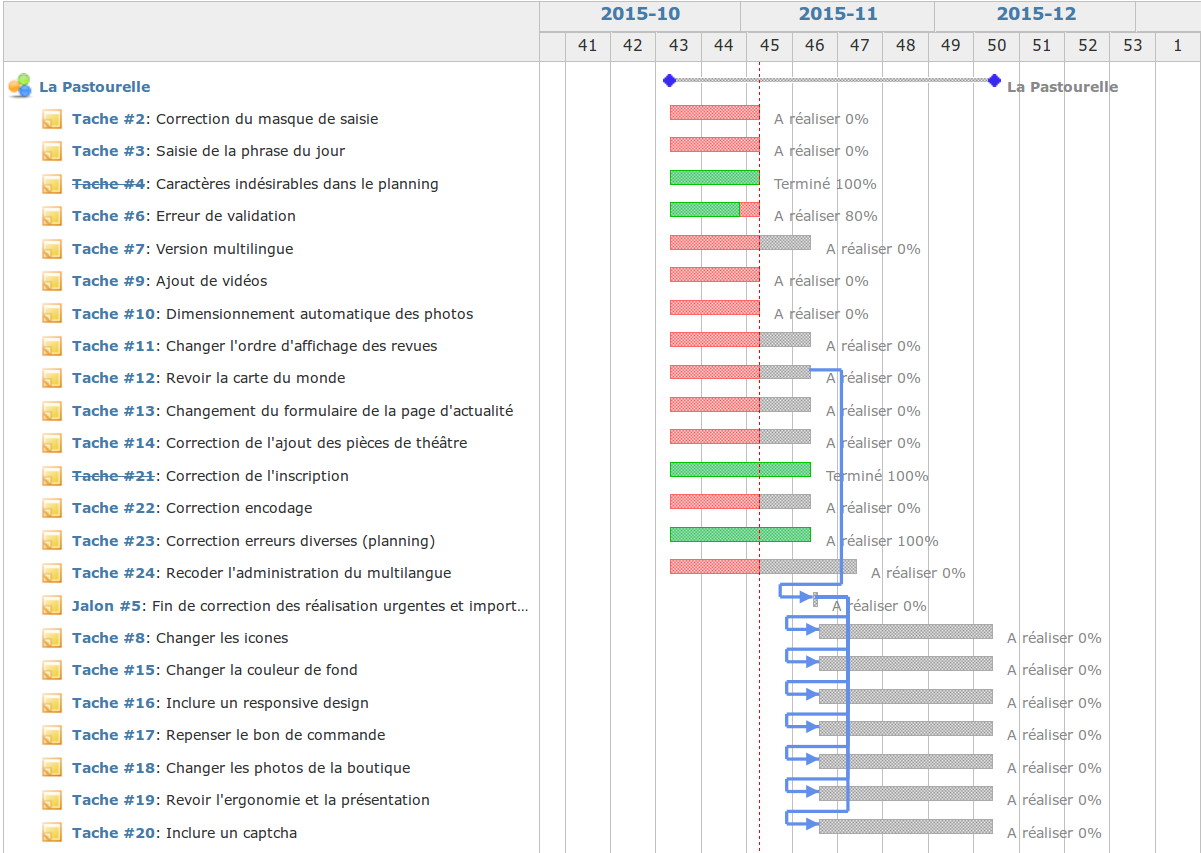
\includegraphics[scale=0.5]{include/gantt3-11.png}
\end{figure}
\end{landscape}

Au 15 novembre 2015, peu avant la deuxième réunion avec le client, le projet à
avancé : les souhaits initiaux ont presque tous été réalisés, et il ne reste que
quelques détails pour finir de coder le multilinguisme.
\par Toutefois, le travail a été très mal organisé car seul Cyril a touché au
code du site à ce jour ainsi qu'à la base de donnée. Notons que nous avons du
refaire la conception de la base de donnée et passer tout le code source en MVC. Par
ailleurs, Clément et Mickael ont réalisé l'étude de l'existant en vu de proposer
au client une nouvelle charte graphique, plus neuve et plus fonctionnelle.
\par Ainsi, le retard que nous avions accumulé a été en grande partie rattrapé,
mais comme nous le voyons au fûr et à mesure de l'avancée de nouvelles tâches se
rajoutent quand nous détectons des problèmes à résoudre. Notons que nous avons
retiré de ce tableau les tâches terminée lors de la plannification précédente :
\begin{tabular}{ | c | p{4cm} | c | c | c | c | c | c |  }
\hline 
Id & Tâche & Statut & Priorité & Estimée (h) & Début & Fin & Réalisé . \\ \hline

%prio urgente %

22 & Correction encodage & Terminée & Urgente & 5 & 21/10/15 & 11/11/15 & 100\%
	  \\ \hline
3 & Saisie de la phrase du jour & Terminée & Urgente & 2 & 21/10/15 & 03/11/15
	& 100\%  \\ \hline
2 & Correction du masque de saisie & Terminée & Urgente & 3 & 21/10/15 &
	03/11/15 & 100\%  \\ \hline
	
%prio haute %	
32 & Correction des erreurs sur le front office & A réaliser & Haute & 3
	& 15/11/2015 & 18/11/2015 & 0  \\ \hline
28 & Modification de base de donnée & Terminée & Haute & 5 & 09/11/15 & 18/11/15
& 100\%  \\ \hline
27 & Retrait de Flash & Terminée & Haute & 10 & 07/11/15 & 18/11/15 & 100\%
 \\ \hline
25 & Ménage & Terminée & Haute & 2 & 05/11/15 & 18/11/15 & 100\%
 \\ \hline
14 & Correction de l'ajout des pièces de théâtre & A réaliser & Haute & 2 &
	13/11/15 & 09/12/15 & 0  \\ \hline
13 & Changement du formulaire de la page d'actualité & Terminée & Haute & 3 &
	21/10/15 & 11/11/15 & 0  \\ \hline
12 & Revoir la carte du monde & A réaliser & Haute & 3 & 21/10/15 & 11/11/15 & 0
	 \\ \hline
11 & Changer l'ordre d'affichage des revues & A réaliser & Haute & 1 & 21/10/15
	& 11/11/15 & 0  \\ \hline
10 & Dimensionnement automatique des photos & A réaliser & Haute & 1 & 21/10/15
	& 03/11/15 & 0  \\ \hline
9 & Ajout de vidéos & Terminée & Haute & 1 & 21/10/15 & 18/11/15 & 100\%  \\
\hline
7 & Version multilingue & A réaliser & Haute & 20 & 21/10/15 & 03/11/15 & 80\% 
\\
\hline
6 & Erreur de validation & Terminée & Haute & 3 & 21/10/15 & 03/11/15 & 100\%
 \\ \hline



%prio moyenne%
31 & Gestion des revues et des pages & Terminée & Moyenne & 2 & 15/11/2015
	& 18/11/2015 & 100\%  \\ \hline
30 & Recoder la partie des comptes rendus & Terminée & Moyenne & 2 & 13/11/2015
	& 18/11/2015 & 100\%  \\ \hline
29 & Recoder la boutique & A réaliser & Moyenne & 2
	& 12/11/2015 & 18/11/2015 & 0  \\ \hline
26 & Correction d'erreurs dans le back office & A réaliser &
Moyenne & 20 & 05/11/2015 & 18/11/2015 & 0  \\ \hline
24 & Recoder l'administration du
	multilangue & A réaliser & Moyenne & 3 & 21/10/15 & 18/11/15 & 0  \\ \hline
	
%prio basse%	
20 & Inclure un captcha & A réaliser & Basse & 2 & 13/11/15 &
	09/12/15 & 0  \\ \hline
19 & Revoir l'ergonomie et la présentation & A réaliser & Basse & ? & 13/11/15
	& 09/12/15 & 0  \\ \hline
18 & Changer les photos de la boutique & A réaliser & Basse & ? & 13/11/15 &
	09/12/15 & 0 \\ \hline
17 & Repenser le bon de commande & A réaliser & Basse & ? & 13/11/15 & 09/12/15
	& 0  \\ \hline
16 & Inclure un responsive design & A réaliser & Basse & ? &
	13/11/15 & 09/12/15 & 0  \\ \hline
15 & Changer la couleur de fond & A réaliser & Basse & ? & 13/11/15 & 09/12/15
	& 0   \\ \hline
8 & Changer les icones & A réaliser & Basse & ? & 21/10/15 & 09/12/15 & 0 \\
\hline

% Total %
 & Total estimé &  &  & 101 &  &  &  \\ \hline
 \end{tabular}
\begin{landscape}
\begin{figure}[t]
    \caption{Avancement du projet au 15 novembre 2015}
   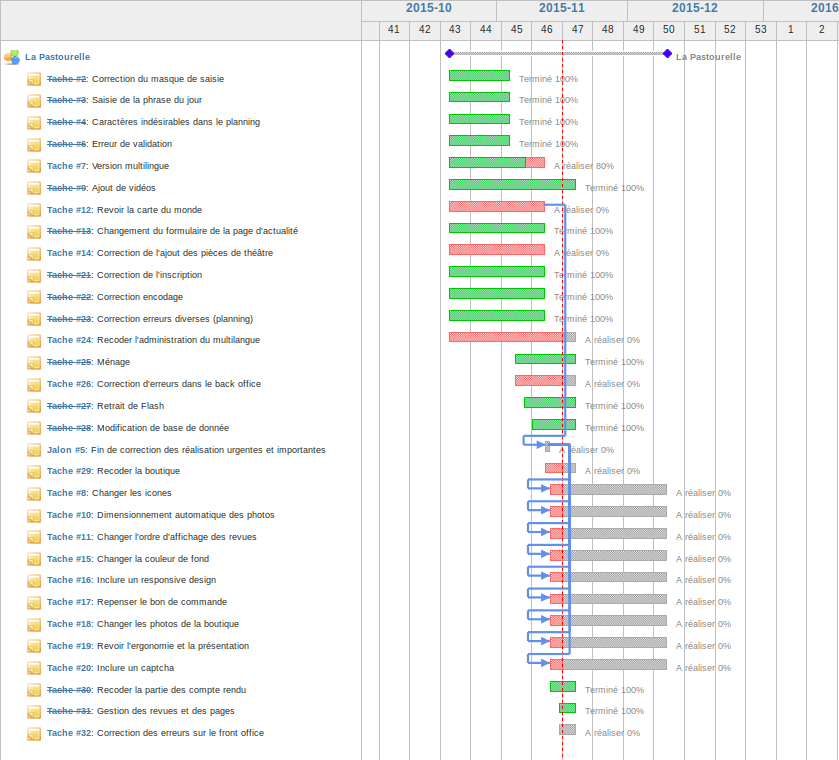
\includegraphics[scale=0.5]{include/gantt15-11.png}
\end{figure}
\end{landscape}

\subsection{Avancement final}

\section{Compte rendu de réunion}
\subsection{Réunion initiale avec le client (21/10/2015)}
Lors de la réunion initiale avec le client, nous lui avons fait part de nos 
interrogations sur les tâches à réaliser. Ainsi, Mr Pagès nous a indiqué que les
plus gros problèmes étaient situés sur les outils de back-office, en raison de 
l'âge du site mais aussi des équipes de développeurs qui se sont succédées pour
le réaliser. \\
\par En ce qui concerne la partie multilangue, il faut conserver les photos
indépendamment de la langue d'utilisation de façon à ne pas devoir les ajouter
n-fois. Pour ce qui est de l'occitan, la traduction des textes sera fournie.
Le masque de saisie est également un gros soucis, car il empêche
l'administrateur de voir le texte saisit, on ne voit que l'équivalent d'un
champ texte, il faut donc agrandir la zone afin d'éviter de devoir faire des
copier/coller depuis Word. \\
\par Pour la boutique, il faut intégrer les nouvelles photos qui seront
fournies, et refaire la présentation du bon de commande sur Word ou un outil
équivalent. Pour la saisie de la phrase du jour, il y a un problème de saisie
directe qui fait que les modifications ne sont pas toujours prises en compte,
sauf si l'on copie/colle depuis un traitement de texte. \\
\par Il faut également revoir la carte du monde qui a des soucis de
duplications, et qui n'est pas pratique du tout à utiliser. Mr Pagès nous a proposé
d'éventuellement changer sa forme ou ne plus utiliser une carte, mais plutôt
des listes ou des tableaux. Pour le planning, il y a un soucis au niveau de la
modification et de la suppression d'un événement contenant des caractères
douteux dans le titre qui empêchent la modification et la suppression, il faut
donc vérifier le filtrage des caractères pour résoudre le problème. \\
\par Si nous avons le temps, le responsable souhaite que nous améliorons le code
CAPTCHA car le site a subit des attaques de robot dans le passé.
La saisie d'actualité doit également être modifiée, il faudrait passer de 5/6
zones textes à une seule en retirant celles qui sont inutiles.
Enfin, il y a un problème avec les picèes de théâtre qui passent à "Pièce
jouée" dès que l'on saisit une valeur, il faudrait donc réparer ce module.

\chapter{Analyse de l'existant}
\chapter{Les caractéristiques techniques}
\section{Charte graphique}
// TODO nouvelle charte graphique
\section{Choix techniques}
\subsection{Slick}
Nous avons utilisé le module Slick, qui est un carroussel codé en jQuery, afin
de proposer un diaporama fluide, efficace et personnalisable. Ainsi, que ce soit
le diaporama du fil d'actualité, celui de l'administration des images, ou encore
celui en haut à droite du site, il seront tous basés sur Slick car le système
actuel est complexe et mal optimisé.

\subsection{TinyMCE}
Le module TinyMCE permet de proposer un éditeur de texte enrichit dans la mesure
où il est possible d'ajouter simplement des images, des vidéos, des liens ou
encore de faire de la mise en page. Il convient très bien pour une utilisation
quotidienne et permettra au client de concevoir ses pages de manière rapide et
en voyant ce qu'il fait car c'est un éditeur type \og WYSIWYG \fg{} (\og what you
see is what you get \fg{}).

\subsection{Bootstrap}
Afin de gagner du développement avec le développement de l'aspect graphique,
nous avons utilisé le template Bootstrap, qui met une large gamme d'outils à
notre disposisions, notamment en ce qui concerne le responsive design et la
gestion des menus. \\
\par Toutefois, afin de proposer des menus déroulants à plusieurs niveaux, nous
avons du le coupler à \og smartmenus \fg{} qui propose des fonctionnalités plus
avancées pour les menus et les onglets déroulants.
\section{Développement}
\subsection{Eléments de sécurisation du site}
Afin d'éviter l'injection SQL, nous avons utilisé PDO avec des requêtes
préparées, ainsi qu'un contrôle des formulaires en amont via PHP et Javascript
pour limiter au maximum les soucis. \\
\par Nous avons aussi refait le système de connexion et de gestion des droits
qui étaient défaillant et inflexible. Ainsi maintenant un membre connecté mais
en attente de validation par un administrateur ne pourra pas accéder au contenu
disponible pour les membres validés, comme c'était le cas avant. Pour ce qui est
des droits d'accès, nous avons augmenté la flexibilité à l'aide d'un système
numérique, ainsi un simple opérateur \og > \fg{} permet de définir le niveau
d'autorisation. Par exemple, si le niveau du membre est \og > 1 \fg{}, il ne
pourra pas accéder aux modules d'administration. \\
 \par Egalement, nous avons mis à jour le système de protection anti-robot, avec
 le système reCaptcha de google, plus facile à utiliser et surtout libre 
 d'utilisation.
 
 \subsection{Codes sources}
 Les codes sources de l'application sont à téléchargés depuis GitHub :
 https://github.com/demmonx/LaPastourelle

\section{Base de données}
Nous avons dû revoir l'intégralité de la base de donnée du site, car c'est un
des élements qui mettait en péril les fonctionnalités du site web. En effet, les
clés primaires définies étaient des champs varchar, du coup le passage de valeur
dans l'URL engendrait des problèmes et il était impossible de traiter
convenablement les données. \\

\par Pour y remédier, nous avons refait une conception de la base de donnée, en
rajoutant les contraintes d'intégrité qui n'étaient pas présente initialement
(clé étrangères, unicité, check). Vous trouverez ce document à la page suivante.
\\

\par En ce qui concerne le choix du SGBD, nous avions le choix entre MySQL et
PostgreSQL, mais notre choix s'est porté sur PostgreSQL pour de multiples
raisons : \\
\begin{itemize}
  \item Les contraintes d'intégrités sont mieux gérées que sur MySQL
  \item Il se rapproche plus d'une utilisation professionnelle, en étant à la
  fois OpenSource, libre et avec de très performances
  \item Il est plus facile à utiliser : l'interface d'administration est mieux
  pensé, l'importation en ligne de commande est plus aisée \\
\end{itemize}

\par Par conséquent, nous avons du nous former à PostgreSQL, ce qui n'était pas
bien compliqué car en dehors de quelques éléments syntaxique qui changent de
MySQL (types, restrictions sur les noms table), le reste était similaire en tout
point.

\chapter{Le déploiement de l'application Web}
\section{Scénarios de recette}
\section{Manuel utilisateur}
\section{Manuel administrateur}
\section{Référencement}
En ce qui concerne le référencement, nous avons simplement rajouté une
description afin que celle-ci apparaisse lors d'une recherche sur un moteur,
sous le titre. Afin d'améliorer le référencement, nous conseillons aux
responsables de l'assocation de multiplier les partenariats, car pour améliorer
le référencement de son site il suffit que son URL soit présente un grand nombre
de fois sur Internet.

\section{Hébergement et compte}
Le site est hébergé sur OVH. Pour accéder au compte et pouvoir sauvegarder ou
restaurer la base de données, les identifiants sont : \\
\begin{itemize}
  \item ID : PC29352-OVH
  \item Mot de passe : CROUZADO \\
\end{itemize}

\par En ce qui concerne la base de données, les informations sont : \\
\begin{itemize}
  \item Utilisateur : pastourebd2
  \item Base de donnée : pastourebd2
  \item Mot de passe :  postgresql84-1.pro
  \item Serveur : ik4FgR12zEgD \\
\end{itemize}

\par Enfin pour le FTP : \\
\begin{itemize}
  \item Utilisateur : pastoure
  \item Mot de passe :  tQWTEXQj
  \item Serveur : ftp.pastourelle-rodez.com
\end{itemize}


\section{Procédure d'archivage}
Idéalement, il faudrait tous les mois sauvegarder la base de données contenant
l'ensemble des informations de l'association, ainsi que les fichiers du site
web, afin de ne pas perdre les modifications apportées sur les ressources
(images, audio).

Pour cela, commençons par copier les fichiers du site  : 
\begin{itemize}
  \item Connectez vous sur le FTP du site via les identifiants donnés dans la
  section précédente, en utilisant le logiciel FileZilla ou équivalent.
  \item Copiez le dossier \og www \fg{} depuis le FTP sur votre ordinateur
  personnel, et précisez la date de la copie. \\
\end{itemize}

\par Ensuite, nous allons nous occuper de copier la base de données. La
manipulation est plus complexe qu'au-dessus : 
\begin{itemize}
  \item Rendez-vous sur le site : https://phppgadmin.ovh.net/
  \item Saisissez les identifiants donnés dans la section précédente
  \item Cliquez sur \og Exporter \fg{}
  \item Choisissez sur \og Structure et données \fg{}
  \item Selectionnez le format \og SQL \fg{}
  \item Prenez l'option \og Exporter \fg{} au lieu de \og Voir \fg{}
  \item Validez en appuyant sur \og Exporter \fg{}
  \item Enregistrez le fichier sur votre ordinateur personnel en précisant la
  date de la copie
\end{itemize}

\section{Procédure de reprise après panne}
En cas de panne importante du site Web, par exemple si une personne mal
intentionnée arrive à supprimer des fichiers ou des informations dans la base de
donnée, il va être nécessaire de restaurer l'état du site à une version
antérieur, fonctionnelle. \\
\par \textbf{Attention toutefois, cela engendrera une perte
des modifications réalisées depuis la dernière sauvegarde}, d'où l'intérêt de
sauvegarder régulièrement. \\

\par Pour restaurer les fichiers du site Web : 
\begin{itemize}
  \item Connectez vous sur le FTP du site via les identifiants donnés dans la
  section précédente, en utilisant le logiciel FileZilla ou équivalent.
  \item Supprimez le contenu du dossier \og www \fg{}
  \item Copiez le contenu du dossier de sauvegarde voulu, situé sur votre
  ordinateur dans le dossier \og www \fg{} du FTP. \\
\end{itemize} 

\par Pour restaurer la base de donnée : 
\begin{itemize}
  \item Rendez-vous sur le site : https://phppgadmin.ovh.net/
  \item Saisissez les identifiants donnés dans la section précédente
  \item Dans le menu de gauche, cliquez sur les \og + \fg{} de manière à voir
  apparaitre l'onglet \og Tables \fg{} et sélectionnez le
  \item Cochez toutes les cases et faites \og Supprimer \fg{} depuis le menu
  d'action
  \item Cochez la case \og CASCADE \fg{} et confirmer la suppression
  \item  Dans le menu de gauche, cliquez sur les \og pastourebd2 \fg{}
  \item Cliquez sur \og SQL \fg{} dans le menu principal (2ème onglet)
  \item Renseignez le fichier à importer, en dessous du champ texte, il
  correspond à la sauvegarde de la base de donnée que vous voulez restaurer
  \item Cliquez sur \og Lancer \fg{} et attendre qu'une nouvelle pas s'affiche,
  avec un certain nombre d'information sur ce qui a été importé \\
\end{itemize}

\par A partir d'ici, le site est de nouveau opérationnel

\section{Conformité du site aux lois en vigueur}
Le site Web est déployé avec des polices typographiques et des icones provenant
de font-awesome, une librairie d'icones et de polices vectorielles sous licence
GPL et libre utilisation pour un projet professionnel et amateur. \\

\par Pour les images hébergées par la Pastourelle, elle provienne de répétitions
ou de concert, et ne dépendent par de la conception du site Web, mais du contenu
qu'en a fait le client. Par conséquent, nous supposons que pour les photos qui
seront hébergées, une demande de droit à l'image aura été préalablement effctuée
auprès des ayant droits. \\

\par Pour les deux modules utilisés, à savoir Slick et TinyMCE, Slick est sous
licence MIT, qui donne le droit de modification, utilisation, etc pour une
utilisation amateure et commerciale du module. TinyMCE est en revanche sous
licence LGPL pour sa version Community, c'est à dire qu'on peut l'utiliser pour
un but commercial ou amateur, mais il y a des restrictions concernant la
modification et la diffusion des codes sources. \\

\par Le template Bootstrap que nous utilisons est sous licence MIT tout comme
son plugin smartmenus, par conséquent nous avons le droit d'utiliser, modifier
et diffuser quelque qu'en soit la finalité. \\

\par Le système anti-robot reCaptcha est placé sous licence CreativeCommons 3.0,
ainsi nous sommes libres de modifier, utiliser et diffuser le module. \\

\par Concernant les logos (tout ce qui touche à la Pastourelle), ils ont été
redéssinés sous Photoshop afin d'ajouter la transparence qui n'était pas
présente. Enfin pour les drapeaux de langues, il faudrait en utiliser sous
licence GPL, qui seront récupérés par le client sur Internet en fonction des
langues qu'il souhaite rendre disponible sur son site.

\section{Support d'archivage}
Le site et la base de données seront fournis sur CD au client tel qu'ils
ont été déployés lors de la phase de mise en production.

\end{document}